%%%%%%%%%%%%%%%%%%%%%%%%%%%%%%%%%%%%%%%%%%%%%%%%%%%%%%%%%%%%%%%
%
% Welcome to Overleaf --- just edit your article on the left,
% and we'll compile it for you on the right. If you give 
% someone the link to this page, they can edit at the same
% time. See the help menu above for more info. Enjoy!
%
%%%%%%%%%%%%%%%%%%%%%%%%%%%%%%%%%%%%%%%%%%%%%%%%%%%%%%%%%%%%%%%
%
% For more detailed article preparation guidelines, please see:
% http://f1000research.com/author-guidelines

\documentclass[10pt,a4paper,twocolumn]{article}
\usepackage{f1000_styles}

%% Default: numerical citations
\usepackage[numbers]{natbib}

%% Uncomment this lines for superscript citations instead
% \usepackage[super]{natbib}

%% Uncomment these lines for author-year citations instead
% \usepackage[round]{natbib}
% \let\cite\citep

\begin{document}

\title{\textit{F1000Research} Article Template}
\titlenote{The title should be detailed enough for someone to know whether the article would be of interest to them, but also concise. Please ensure the broadness and claims within the title are appropriate to the content of the article itself.}
\author[1]{Author Name1}
\author[2]{Author Name2}
\affil[1]{Address of author1}
\affil[2]{Address of author2}

\maketitle
\thispagestyle{fancy}

Please list all authors that played a significant role in the research involved in the article. Please provide full affiliation information (including full institutional address, ZIP code and e-mail address) for all authors, and identify who is/are the corresponding author(s).

\begin{abstract}

Abstracts should be up to 300 words and provide a succinct summary of the article. Although the abstract should explain why the article might be interesting, care should be taken not to inappropriately over-emphasize the importance of the work described in the article. Citations should not be used in the abstract, and the use of abbreviations should be minimized. If you are writing a Research or Systematic Review article, please structure your abstract into Background, Methods, Results, and Conclusions.


\end{abstract}

\section*{Keywords}

Please list up to eight keywords to help readers interested in your article find it more easily.

\clearpage

\section*{Introduction}

The format of the main body of the article is flexible: it should be concise and in the format most appropriate to displaying the content of the article.

Some examples of commonly used \LaTeX{}  commands and features are listed below, to help you get started.


\subsection*{Sections}

Use section and subsection commands to organize your document. \LaTeX{} handles all the formatting and numbering automatically. Use ref and label commands for cross-references.


\subsection*{Tables}

Use the table and tabledata commands for basic tables --- see Table~\ref{tab:widgets}, for example.
\begin{table}[h!]
\hrule \vspace{0.1cm}
\caption{\label{tab:widgets}An example of a simple table with caption.}
\centering
\begin{tabledata}{llr} 
\header First name & Last Name & Grade \\ 
\row John & Doe & $7.5$ \\ 
\row Richard & Miles & $2$ \\ 
\end{tabledata}
\end{table}

\subsection*{Figures}
You can upload a figure (JPEG, PNG or PDF) using the files menu. To include it in your document, use the includegraphics command (see the example below in the source code).

Please give figures appropriate filenames eg: figure1.pdf, figure2.png.

Figure legends should briefly describe the key messages of the figure such that the figure can stand alone from the main text. However, all figures should also be discussed in the article text. Each legend should have a concise title of no more than 15 words. The legend itself should be succinct, while still explaining all symbols and abbreviations. Avoid lengthy descriptions of methods.

For any figures reproduced from another publication (as long as appropriate permission has been obtained from the copyright holder —see under the heading 'Submission'), please include a line in the legend to state that: 'This figure has been reproduced with kind permission from [include original publication citation]'.

\begin{figure}
\centering
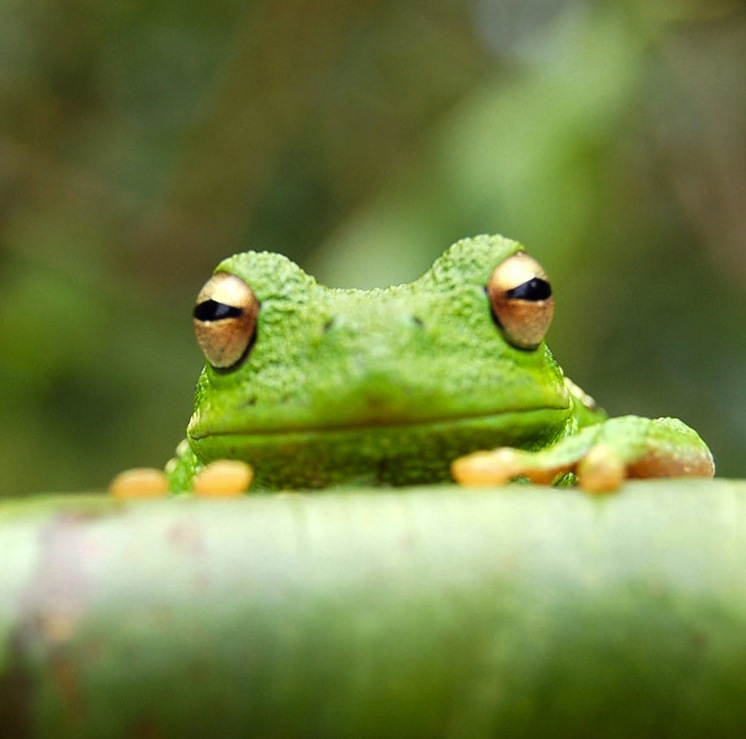
\includegraphics[width=0.4\textwidth]{frog.jpg}
\caption{\label{fig:your-figure}Your figure legend goes here; it should be succinct, while still explaining all symbols and abbreviations. }
\end{figure}



\subsection*{Mathematics}

\LaTeX{} is great at typesetting mathematics. Let $X_1, X_2, \ldots, X_n$ be a sequence of independent and identically distributed random variables with $\text{E}[X_i] = \mu$ and $\text{Var}[X_i] = \sigma^2 < \infty$, and let
$$S_n = \frac{X_1 + X_2 + \cdots + X_n}{n}
      = \frac{1}{n}\sum_{i}^{n} X_i$$
denote their mean. Then as $n$ approaches infinity, the random variables $\sqrt{n}(S_n - \mu)$ converge in distribution to a normal $\mathcal{N}(0, \sigma^2)$.

\subsection*{Lists}

You can make lists with automatic numbering \dots

\begin{enumerate}
\item Like this,
\item and like this.
\end{enumerate}
\dots or bullet points \dots
\begin{itemize}
\item Like this,
\item and like this.
\end{itemize}

\section*{Methods}
Methods should include a brief discussion of allowances made (if any) for controlling bias or unwanted sources of variability, and the limitations of the datasets.


\section*{Results}
This section is not essential for Web Tool papers.

\section*{Discussion}
The discussion should include the implications of the article results in view of prior work in this field.

\section*{Conclusions}
Please state what you think are the main conclusions that can be realistically drawn from the findings in the paper, taking care not to make claims that cannot be supported.



\subsection*{Author contributions}
In order to give appropriate credit to each author of an article, the individual
contributions of each author to the manuscript should be detailed in this section. We
recommend using author initials and then stating briefly how they contributed.

\subsection*{Competing interests}
All financial, personal, or professional competing interests for any of the authors that
could be construed to unduly influence the content of the article must be disclosed and
will be displayed alongside the article.

\subsection*{Grant information}
Please state who funded the work discussed in this article, whether it is your employer,
a grant funder etc. Please do not list funding that you have that is not relevant to this
specific piece of research. For each funder, please state the funder’s name, the grant
number where applicable, and the individual to whom the grant was assigned.
If your work was not funded by any grants, please include the line: ‘The author(s)
declared that no grants were involved in supporting this work.’

\subsection*{Acknowledgements}
This section should acknowledge anyone who contributed to the research or the
article but who does not qualify as an author based on the criteria provided earlier
(e.g. someone or an organisation that provided writing assistance). Please state how
they contributed; authors should obtain permission to acknowledge from all those
mentioned in the Acknowledgements section.

Please do not list grant funding in this section.


{\small\bibliographystyle{unsrtnat}
\bibliography{ref}}

\bigskip
References can be listed in any standard referencing style that uses a numbering system
(i.e. not Harvard referencing style), and should be consistent between references within
a given article.

Reference management systems such as Zotero provide options for exporting bibliographies as Bib\TeX{} files. Bib\TeX{} is a bibliographic tool that is used with \LaTeX{} to help organize the user's references and create a bibliography. This template contains an example of such a file, \texttt{sample.bib}, which can be replaced with your own. Use the \verb|\cite| command  to create in-text citations, \cite{zheng2017massively}
%like this \cite{Smith:2012qr} and this \cite{Smith:2013jd}.


% See this guide for more information on BibTeX:
% http://libguides.mit.edu/content.php?pid=55482&sid=406343

% For more author guidance please see:
% http://f1000research.com/author-guidelines


% When all authors are happy with the paper, use the 
% ‘Submit to F1000Research' button from the menu above
% to submit directly to the open life science journal F1000Research.

% Please note that this template results in a draft pre-submission PDF document.
% Articles will be professionally typeset when accepted for publication.

% We hope you find the F1000Research Overleaf template useful,
% please let us know if you have any feedback using the help menu above.


\end{document}